\documentclass[border=5pt]{standalone}
\usepackage{tikz}
\usetikzlibrary{arrows}
\begin{document}

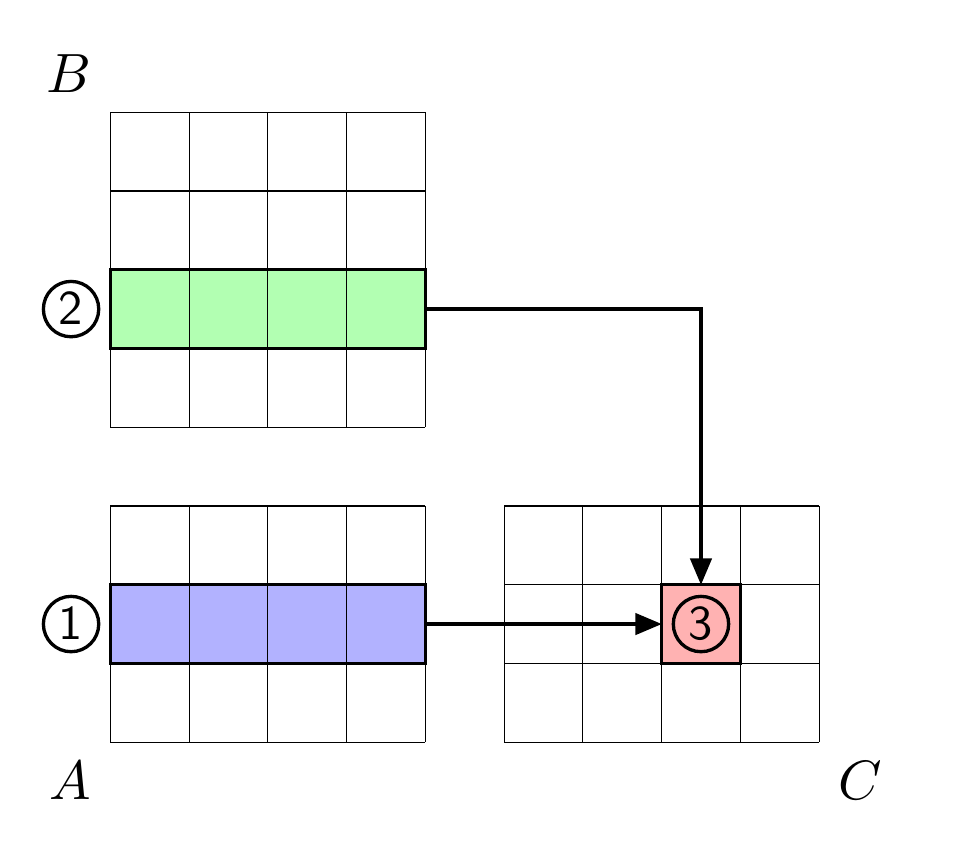
\begin{tikzpicture}[node distance=0.15 cm, font=\sffamily]

% colored elements
\fill[color=blue!30] (0,1) rectangle (4,2);  % blue row
\fill[color=green!30] (0,5) rectangle (4,6); % green row
\fill[color=red!30] (7,1) rectangle (8,2);   % red element

% matrices
\draw[step=1cm,black,thin] (0,0)grid(4,3); % A
\draw[step=1cm,black,thin] (0,4)grid(4,8); % B
\draw[step=1cm,black,thin] (5,0)grid(9,3); % C

% labels
\node[anchor=north east, scale=2] at (0,0) {$A$};
\node[anchor=south east, scale=2] at (0,8) {$B$};
\node[anchor=north west, scale=2] at (9,0) {$C$};

% invisible label (to have same figure size as allpairs_access_pattern)
\node[color=white, anchor=south west, scale=2] at (9,8) {$B^T$};

\begin{scope}[very thick]	
	% boxes around colored elements
	\draw (0,1) rectangle (4,2); % green row
	\draw (0,5) rectangle (4,6); % blue row
	\draw (7,1) rectangle (8,2); % red element
	
	% arrows
	\draw[->,>=triangle 45] (4,5.5) -- (7.5,5.5) -- (7.5,2);
	\draw[->,>=triangle 45] (4,1.5) -- (7,1.5);
\end{scope}

\node[draw, circle, minimum size=20pt, line width=1.2] (rowA) at (-0.5,1.5) {};
\node[scale=1.75] at (rowA.center) {1};

\node[draw, circle, minimum size=20pt, line width=1.2] (rowB) at (-0.5,5.5) {};
\node[scale=1.75] at (rowB.center) {2};

\node[draw, circle, minimum size=20pt, line width=1.2] (elementC) at (7.5,1.5) {};
\node[scale=1.75] at (elementC.center) {3};
    
\end{tikzpicture}
\end{document}
